% Define center type column
\newcolumntype{Y}{>{\centering\arraybackslash}X}
\newcolumntype{P}[1]{>{\centering\arraybackslash}m{#1}}
\newcolumntype{T}[1]{>{\small\centering\arraybackslash}m{#1}}
\renewcommand\tabularxcolumn[1]{m{#1}}

%spacing
\renewcommand{\arraystretch}{2}
\begin{table}
    \small
    \begin{tabularx}{\textwidth}{T{2.5cm} T{2cm} P{4cm}  Y }
        \small{Matching} & \small{Applications} & Pattern & Text with occurrences underlined \\
        \hline
        Regular expression \cite{RM-704} & & $P=$ GAT$(\mathrm{TA}\mid \mathrm{O})(\mathrm{CAT})^*$ & $T=$~\underline{GATTA}AT\underline{GATOCATCAT}A \\
        %Error bound~\cite{landau1986efficient} (for ED~\cite{levenshtein1966binary}) & $P=$ GATTACAT & $T=$ AT\underline{GATTAACAT}ATA, $\mathrm{ED}(P,T[2..10])=1$ \\
        Don't care \cite{fischer1974string} & & $P=$ GAT**CAT & \underline{GATTACAT}A\underline{GATOACAT}AC\\
        %
        Gapped consecutive \cite{bille2022gapped} & & $P_1=$ GATTA $P_2=$ TAC  $a=2$, $b=6$ & $T=$ AGG\underline{GATTAC}TAC, distance between $P_1$ and $P_2$ $d=3 \in [a,b]$\\
        %
        Degenerate \cite{abrahamson1987generalized}  & & $P=$ GATTACAT &  $T=$ {\renewcommand{\arraystretch}{1} A$\left\{
            \begin{array}{l}
                \mathrm{T}  \\
                \mathrm{C}
            \end{array}\right\}$\underline{GAT}$\left\{
            \begin{array}{l}
                \mathrm{\underline{T}}  \\
                \mathrm{A}
            \end{array}\right\} \mathrm{\underline{ACAT}A}$} \\
        %
        %
        Elastic degenerate \cite{iliopoulos2021efficient}  & & $P=$ GATTACAT &  $T=$ {\renewcommand{\arraystretch}{1} AT\underline{GAT}$\left\{
            \begin{array}{l}
                \mathrm{\underline{TA}}  \\
                \mathrm{A}
            \end{array}\right\} \mathrm{\underline{CAT}A}$} \\
        %
        Generalised degenerate \cite{alzamel_et_al:LIPIcs:2018:9323}  & & $P=$ GATTACAT &  $T=$ {\renewcommand{\arraystretch}{1} AT$\left\{
            \begin{array}{l}
                \mathrm{\underline{G}}  \\
                \mathrm{T}
            \end{array}\right\}
        \mathrm{\underline{AT}}\left\{
            \begin{array}{l}
                \mathrm{\underline{TA}}  \\
                \mathrm{AT}
            \end{array}\right\} \mathrm{\underline{CAT}A}$} \\
        %
        Abelian/Jumbled \cite{eres2004permutation} & & $P=$ GATTACAT & $T=$ AGAG\underline{TATGATCA}GT\\
        %
        Weighted \cite{thompson1994clustal} & & GATTA has a cumulative probability $>0.07$. & 
        \begin{minipage}{4.5cm} \footnotesize
            \renewcommand{\arraystretch}{1}
            \begin{tabular}{c|ccccc}
                 & 0    & 1 & 2 & 3 & 4 \\
                \hline
                A & 0    & \underline{1} & 0.25 & 0 & \underline{0.75}\\
                C & 0.25 & 0 & 0.25 & 0 & 0.25\\
                G & \underline{0.75} & 0  & 0.25 & 0.5 & 0\\
                T & 0    & 0  & \underline{0.25} & \underline{0.5} & 0\\
            \end{tabular}
        \end{minipage} \\
        %
        Order preserving \cite{kim2014order,kubica2013linear} & & $P =$ 1 5 3 4 6 2 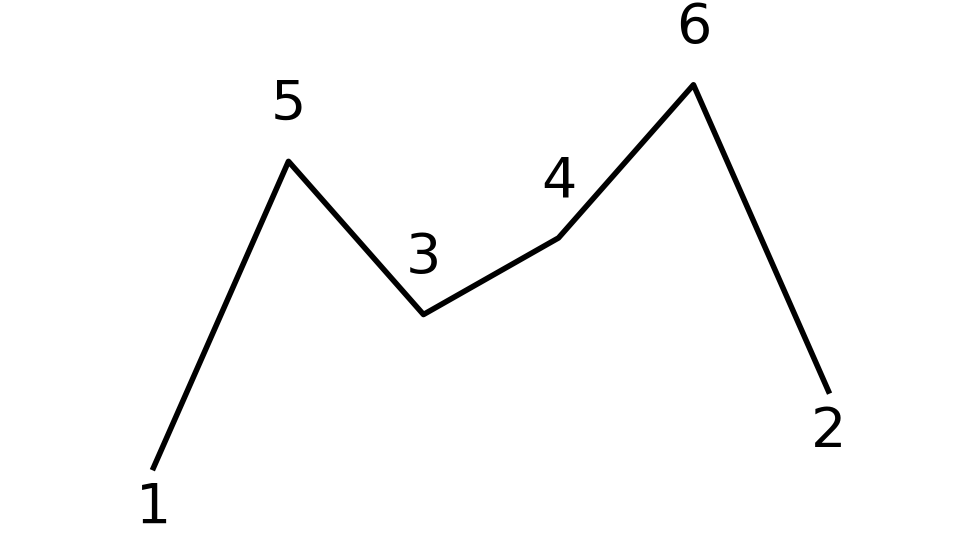
\includegraphics[width=3cm]{Introduction/op_P.png} & $T=$ \underline{2 7 4 5 8 3} \underline{1 20 15 16 25 6}  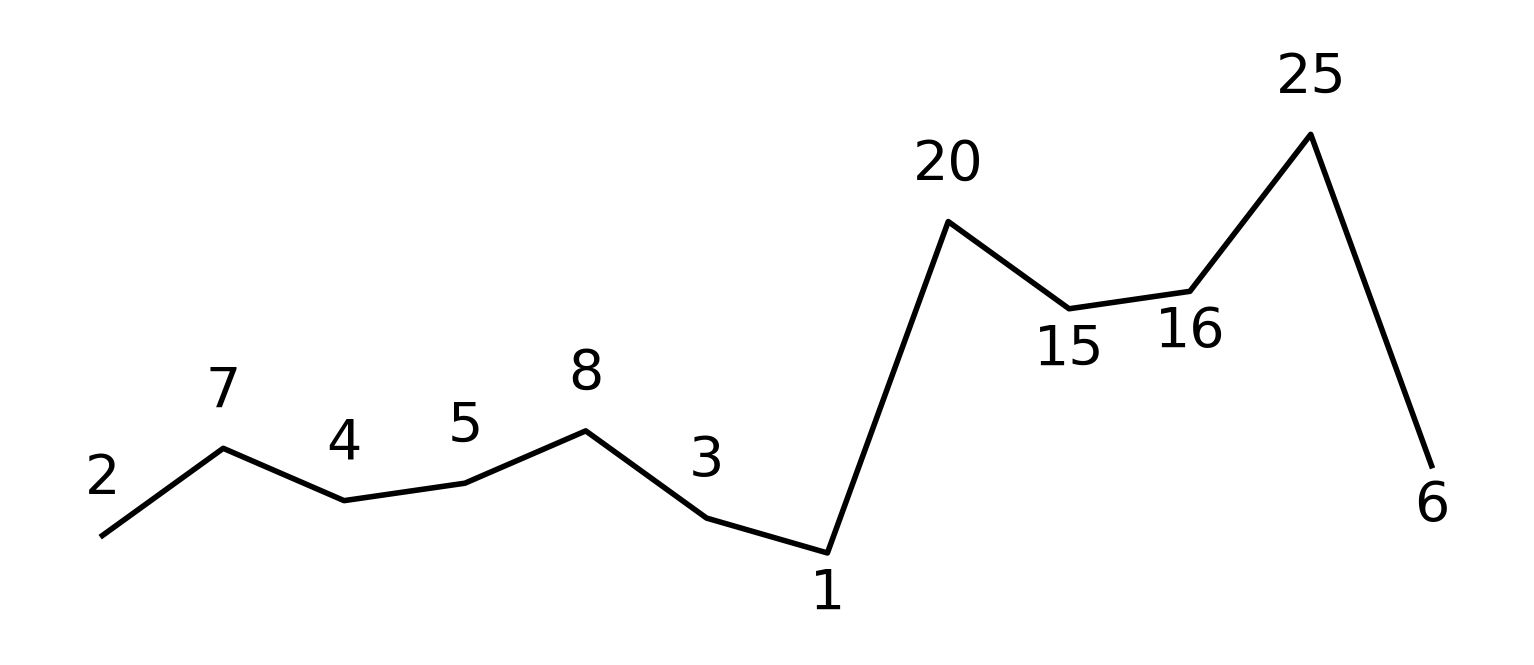
\includegraphics[width=5cm]{Introduction/op_T.png} \\
        %
        Parametrized \cite{baker1993theory} & & $P=$ GATTACAT & $T=$ OPO\underline{POGGODOG}O, \begin{minipage}{3cm} A:O, C:D, G:P, T:G \end{minipage} \\
    \end{tabularx}
    \caption{Example of various model of matching on strings.}
    \label{fig:intro:match_model}
\end{table}